\documentclass{beamer}
\usepackage{amsmath,amssymb,amsfonts,latexsym,stmaryrd}
\usepackage[utf8]{inputenc}
\usepackage[spanish]{babel}
\usepackage{graphicx}
\usepackage[ruled,vlined,lined,linesnumbered,algosection,spanish]{algorithm2e}
\usepackage[T1]{fontenc}
\usepackage{verbatim}
\usepackage{verbments}
\usepackage{marvosym}
\usepackage[marvosym]{tikzsymbols}
\definecolor{fondo1}{rgb}{0.96, 0.96, 0.96}
\definecolor{fondo2}{rgb}{0.3, 0.6, 0.5}
\usefonttheme{professionalfonts} % fuentes de LaTeX
\usetheme{Cyberjaya}
\usepackage{lipsum}             % for dummy text
%\setbeamercovered{transparent} % Velos
%\setbeamertemplate{footline}{}
%\titlegraphic{aster.jpeg}
%Define el color del fondo de la imagen
%\titlegraphicbackground{usydred}
\title{Escritura básica de textos}
\subtitle{Parte I}
\author[HeNeos]{Josué Huaroto Villavicencio}
\begin{document}
\fvset{frame=bottomline, framerule=0.02cm}
\plset{language=latex,texcl=true, listingnamefont=\sffamily\bfseries\color{white},captionbgcolor=fondo2, bgcolor=fondo1,listingname=\textbf{Iniciando}, captionfont=\sffamily\color{white}}
\begin{frame}
\maketitle
\end{frame}
\section{Clases de documentos}
\begin{frame}{Clases de documentos}
Antes de empezar a escribir algo, debemos saber que tipo de documento vamos a realizar$\ldots$ ¿se tratará de un informe, artículo, revista, libro, carta, reporte,etc.?\\[20pt]
\textbf{\large ¿Por qué es importante esto?}\\[6pt]
Como se explicó en la parte introductoria, \LaTeX \, nos permite centrarnos en el contenido del documento para no perder tiempo en aspectos estéticos de éste; sin embargo, para que \LaTeX \, pueda darle un aspecto visualmente atractivo a nuestro documento depende de algunos parámetros que podemos brindarle; uno de ellos es el tipo de documento, pues \LaTeX \, organizará la información de distintas formas según si el documento es un \texttt{article, report, book, beamer} o \texttt{letter}. En el curso trabajaremos principalmente con \texttt{article, report} y en las últimas clases con \texttt{beamer}.
\end{frame}
\begin{frame}[fragile]
\frametitle{Clases de documentos}
\framesubtitle{¿Y cómo indico cuál documento quiero?}
Empezamos con las clases de documentos porque además de ser muy útil para idear y planificar cómo se verá nuestro documento, también es un paramétro \textbf{obligatorio} que debemos pasarle a \LaTeX \, para iniciar a escribir.\\[10pt]
Es decir, nuestra primera línea de código en \LaTeX \, será la declaración del tipo de documento:
\begin{pyglist}[language=latex,caption={Clase del documento},style=rainbow_dash]
\documentclass[...]{article}
\end{pyglist}
\end{frame}
\begin{frame}[fragile]
\frametitle{Clases de documentos}
\framesubtitle{¿Puedo agregar más opciones?}
La opción dentro de [ ] es lo que se conoce formalmente como un parámetro, la mayoría de veces son opcionales y \LaTeX \, toma uno por defecto si no lo especificamos; en este caso podemos introducir dentro algunas opciones como:
\begin{pyglist}[language=latex,caption={Clase del documento y parámetro},style=rainbow_dash]
\documentclass[a4paper,12pt]{article}
\end{pyglist}
Aquí hemos espeficicado que nuestro documento sera del tipo artículo y tendrá un formato A4 y de tamaño de letra de 12pt.
\end{frame}
\begin{frame}[fragile]
\frametitle{Clases de documentos}
\framesubtitle{¿Y ahora qué...?}
Vale, probablemente estés inquieto para ya empezar a escribir tu primer texto en \LaTeX. Para ello vamos a mostrar un código simple para que ya puedas comenzar a escribir y poco a poco iremos agregando algunas cosas para que esté mejor detallado:
\begin{pyglist}[language=latex,caption={Clase del documento y parámetro},style=rainbow_dash]
\documentclass[a4paper,12pt]{article}
\begin{document} %Inicio del documento
Hola UNI, este es mi primer texto en \LaTeX.
\end{document} %Fin del documento
\end{pyglist}
Okay... el código se ve simple y sencillo de entender, ¿no? El símbolo \% es usado para los comentarios en \LaTeX
\end{frame}
\section{Fuentes, tamaños y colores}
\begin{frame}
\frametitle{Fuentes, tamaños y colores}
\framesubtitle{No encuentro un botón para cambiar la fuente, ahhh aiudaaa}
Don't panic.\\[20pt]
Las fuentes pueden accederse de la siguiente forma:
\begin{columns}[t]
\begin{column}{.58\linewidth}
\begin{block}{Código}
\begin{itemize}
\item \texttt{$\backslash$textrm\{romana normal\} } 
\item \texttt{$\backslash$textsf\{sans serif\} } 
\item \texttt{$\backslash$texttt\{mono-espaciada\} } 
\item \texttt{$\backslash$textit\{cursiva o itálica\} } 
\item \texttt{$\backslash$textbf\{negrita\} } 
\item \texttt{$\backslash$textsl\{inclinada\} } 
\item \texttt{$\backslash$textsc\{versalita\} } 
\end{itemize}
\end{block}
\end{column}
\begin{column}{.38\linewidth}
\begin{block}{Resultado}
\begin{itemize}
\item \textrm{romana normal} 
\item \textsf{sans serif}
\item \texttt{mono-espaciada}
\item \textit{cursiva o itálica}
\item \textbf{negrita}
\item \textsl{inclinada}
\item \textsc{versalita} 
\end{itemize}
\end{block}
\end{column}
\end{columns}
\end{frame}
\begin{frame}
\frametitle{Fuentes, tamaños y colores}
\framesubtitle{No encuentro un botón para cambiar el tamaño, ahhh aiudaaa}
\begin{columns}[t]
\begin{column}{.58\linewidth}
\begin{block}{Código}
\begin{itemize}
\item \texttt{\{$\backslash$tiny} texto\}
\item \texttt{\{$\backslash$scriptsize} texto\} 
\item \texttt{\{$\backslash$footnotesize} texto\}
\item \texttt{\{$\backslash$small} texto\}
\item \texttt{\{$\backslash$normalsize} texto\} 
\item \texttt{\{$\backslash$large} texto\}
\item \texttt{\{$\backslash$Large} texto\}
\item \texttt{\{$\backslash$LARGE} texto\}
\item \texttt{\{$\backslash$huge} texto\}
\item \texttt{\{$\backslash$Huge} texto\}
\end{itemize}
\end{block}
\end{column}
\begin{column}{.38\linewidth}
\begin{block}{Resultado}
\begin{itemize}
\item {\tiny texto} 
\item {\scriptsize texto}
\item {\footnotesize texto}
\item {\small texto}
\item {\normalsize texto}
\item {\large texto}
\item {\Large texto} 
\item {\LARGE texto} 
\item {\huge texto}
\item {\Huge texto}  
\end{itemize}
\end{block}
\end{column}
\end{columns}
\end{frame}
\begin{frame}[fragile]
\frametitle{Fuentes, tamaños y colores}
\framesubtitle{No encuentro un botón para cambiar el color, ahhh aiudaaa}
Esto se soluciona de forma simple con la siguiente instrucción:
\begin{verbatim}
{\color{blue}\LaTeX \ is} cool
\colorbox{red}{\color{white}\LaTeX \ is} cool
\LaTeX \ is {\color{\green}cool}
\fcolorbox{yellow}{cyan}{\color{white}\LaTeX \ is cool}

\setlength{\fboxrule}{2pt}
\fcolorbox{yellow}{cyan}{\color{white}\LaTeX \ is cool}

\setlength{\fboxsep}{6pt}
\fcolorbox{yellow}{cyan}{\color{white}\LaTeX \ is cool}
\end{verbatim}
{\color{blue}\LaTeX \ is} cool
\colorbox{red}{\color{white}\LaTeX \ is} cool
\LaTeX \ is {\color{green}cool}
\fcolorbox{yellow}{cyan}{\color{white}\LaTeX \ is cool}
\setlength{\fboxrule}{2pt}
\fcolorbox{yellow}{cyan}{\color{white}\LaTeX \ is cool}
\setlength{\fboxsep}{6pt}
\fcolorbox{yellow}{cyan}{\color{white}\LaTeX \ is cool}
\end{frame}
\section{Portada simple}
\begin{frame}[fragile]
\frametitle{Portada simple}
Con lo que se te ha explicado hasta ahora podría construir una portada simple... claro, esto probablemente tome mucho tiempo para que al menos quede decente. Don't worry, \LaTeX \ tiene un comando especial para hacer esto de forma rápida:
\begin{pyglist}[language=latex,caption={Portadas simple},style=rainbow_dash]
\documentclass[a4paper,12pt]{article}
\author{Manolito Perez xd :v}
\title{Haciendo una portada simple}
\date{aqui va la fecha pero puedo poner lo que sea xd}
\begin{document}
\maketitle
Hola UNI, este es mi primer texto en \LaTeX.
\end{document}
\end{pyglist}
\end{frame}
\begin{frame}
Compilalo y verás el resultado \Winkey[1.2][yellow].
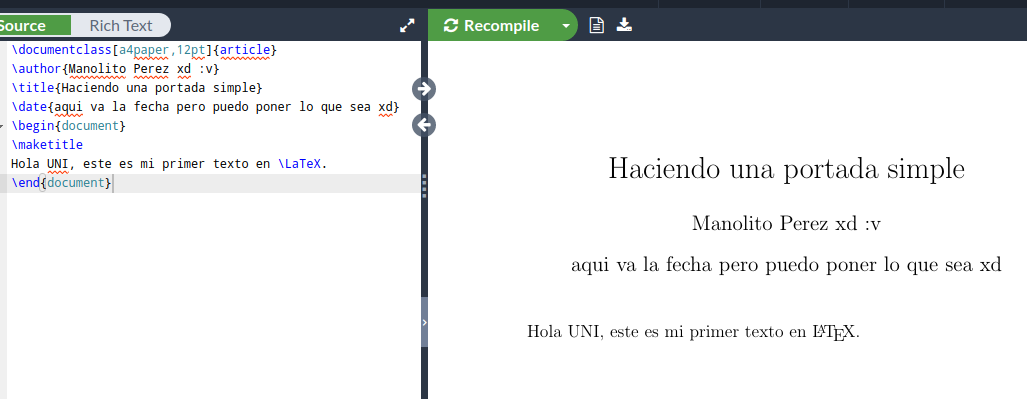
\includegraphics[scale=0.31]{portsimp}
\end{frame}
\end{document}
